\chapter{Synthesis of a Sparse 2D-Scanning Array using Particle Swarm Optimization for Side-Lobe Reduction}
\blfootnote{\textbf{Publication:} S. Goswami, K. Sarmah, K. K. Sarma, and N. E. Mastorakis, ``Synthesis of a Sparse 2D-Scanning Array using Particle Swarm Optimization for Side-Lobe Reduction,'' in proc. \emph{24th International Conference on Circuits, Systems, Communications and Computers}, Crete Island, Greece, July, 2021.\\ (Published in WSEAS Transactions on Communications, vol. 20, p. 112-116, 2021, doi: 10.37394/23204.2021.20.14)}
\label{chap:chap5}
\section{Introduction}\label{c5sec_intro}
A phased array antenna is widely used in wireless communication and radar systems. With the evolution of 5G and millimeter-wave communication, a large grid of small printed antennas is becoming popular \cite{5gmmwave, 5gmmwave_fr4}.

A phased array antenna comprises stationary elements excited at different phases to obtain radiation in different directions \cite{phasedArrayHandbook}. Phased arrays have been there for a long time. The first phased array antenna was made in 1955 \cite{phasedArray_russia}. The first printed phased array was reported by Munson et al. in 1974 \cite{txmPhasedArray}. With the evolution of microwave and millimeter-wave communication standards, the use of phased arrays became more common. There has been extensive research on phased array antennas with a significant number of radiating elements for 5G wireless communication \cite{mmarrayRrev}.

The elements of a typical phased array have a spacing of one-half of the operating wavelength, represented by $\lambda/2$ \cite{phasedArrayHandbook}. A sparse array is a phased array antenna that has fewer elements than a conventional array. The concept of sparse array was introduced in 1962 by R. W. Willey \cite{sparse_rect_planar}. Synthesis of a sparse array reduces the overall cost, weight, required power, dissipated heat, etc. of a communication or a radar system because of the reduced number of elements of the array and the corresponding reduction in the excitation circuitry \cite{sparseDesignConstraints}.

When an array has a fewer number of elements, the spacing between the elements becomes greater than $\lambda/2$. This causes an increase in the number of side lobes of the antenna. This is a major drawback of sparse arrays. Traditionally, this problem was addressed by adjusting the positions, spacing, and excitation weights of the array \cite{sparseDesignConstraints}.

With the advancement of modern computers, soft-computational optimization algorithms are widely being used for the synthesis of sparse arrays. Synthesizing a sparse array from a fully populated array is called an array thinning problem. A solution to an array thinning problem using genetic algorithm was proposed by R. Jain et al. in 2012 \cite{thinningGA}. Another similar work was published by M. A. Zaman et al. in 2012 \cite{nunUniformLinear}. There are also analytical approaches for the synthesis of arrays. In 2016, E. Sandi et al. proposed a technique for the synthesis of sparse arrays using a combination of cyclic difference set and binomial amplitude tapering \cite{amplitudeTaperingHybrid}. Such approaches usually involve a complex mathematical formulation and limited usability.

In recent years, the synthesis of planar sparse arrays is emerging as a popular area of research. A modified genetic algorithm for the synthesis of planar arrays was proposed in 2017 by K. Y. Reddy et al \cite{randomlySpacedArray}. Another multi-objective optimization-based technique for sparse array synthesis was proposed in 2020 by H. Li et al \cite{selfOrgOpt}. In both of these works, the primary objective was to minimize the peak side-lobe power. The radiation pattern of the antenna is calculated numerically to obtain the value of the fitness function. There are also analytical approaches for the synthesis of planar phased array antennas. A singular value decomposition (SVD) based non-iterative approach for array synthesis was reported by P. F. Gu et al. in 2019 \cite{SyntLargeSparse}.

Arrays of printed antennas are most commonly used for millimeter-wave communication. Most of the printed antennas with a ground plane have a cosine radiation pattern. In this work, a sparse 2D phased array is presented with cosine antenna elements. The sparse array is synthesized from a $16\times 16$ uniform rectangular array (URA). The number of elements in the array is reduced by 50\%. The positions of the elements are tuned with Particle Swarm Optimization (PSO) algorithm to minimize the peak side-lobe level (PSLL).

The PSLL, gain and beam-width of the synthesized sparse planar array are compared with the original URA. It is observed that the synthesized sparse array yields a narrower beam-width than the original sparse array. A narrower beam-width is indicative of a better resolution of the scanning array \cite{sparseDesignConstraints}.

The remaining sections of the chapter are arranged as follows. The details of the synthesis and optimization of the sparse array from a $16\times16$ URA are presented in Section \ref{c5sec_design}. This section is followed by the experimental results and discussions in Section \ref{c5sec_res}. The chapter is concluded in Section \ref{c5sec_cncl}.

Matlab Phased Array System Toolbox$^{\circledR}$ is used for computing all radiation patterns used and presented in this work.

\section{Design Details}\label{c5sec_design}
\subsection{Array Topology and Progressive Phase Excitation}
The topology of the uniform rectangular array is shown in Fig. \ref{fig_5_1}. It is a uniform array with a spacing of half of the wavelength ($\lambda/2$) in both directions. The antenna element used is a cosine element.

\begin{figure}
  \centering
  
\includegraphics[width=0.4\linewidth]{Fig-naun_1.eps}\\
  \caption{Topology of the URA} \label{fig_5_1}
\end{figure}

Along the direction of the azimuth plane, the $k^{th}$ element has a phase of $(k-1)\delta_{AZ}$. Similarly, the $m^{th}$ element along the direction of the elevation angle has a phase of $(m-1)\delta_{EL}$. Thus, the weight of excitation of the element $(k, m)$ in the 2D array is given by Eq. \ref{c5_eq1}.

\begin{equation}\label{c5_eq1}
\begin{split}
W & = e^{j(k-1)\delta_{AZ}} \times e^{j(m-1)\delta_{EL}}~=~e^{j[(k-1)\delta_{AZ} + (m-1)\delta_{EL}]} \\
  & = \cos[(k-1)\delta_{AZ} + (m-1)\delta_{EL}] + j\sin[(k-1)\delta_{AZ} + (m-1)\delta_{EL}]
\end{split}
\end{equation}

\begin{figure}
  \centering
  \subfigure[Progressive phase shift in the direction of azimuthal plane]{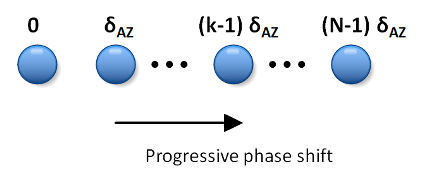
\includegraphics[width=0.4\linewidth]{Fig-naun_2a.eps}} ~~~~
  \subfigure[Progressive phase shift in the direction of azimuthal plane]{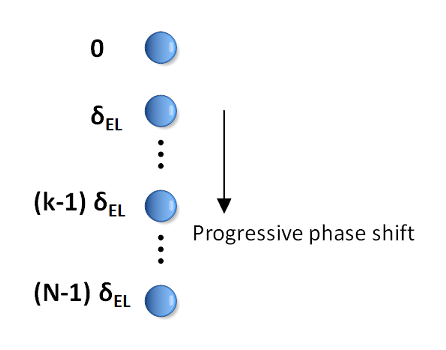
\includegraphics[width=0.4\linewidth]{Fig-naun_2b.eps}}\\
  \caption{Illustration of the progressive phase shift in excitation} \label{fig_5_2}
\end{figure}

The progressive phase shift is illustrated in Fig. \ref{fig_5_2}. For a uniform linear array, the analytical equations are available for estimating the values of the direction of the major lobe from the value of the progressive phase shift ($\delta$) \cite{phasedArrayHandbook}. In this work, an experimental method is used to understand this correlation for the 2D planar array. A dataset is created by varying both $\delta_{AZ}$ and $\delta_{EL}$ within a range of -135 degree to 135 degree at intervals of 15 degree resulting in a total of 361 scan-angles. The direction of the major lobe of the resultant radiation pattern is represented in terms of a combination of the azimuth angle ($\phi$) and the elevation angle ($\theta$) in a 3D polar coordinate system. The correlation plots are shown in Fig. \ref{fig_5_3}.

\begin{figure}
  \centering
  \subfigure[]{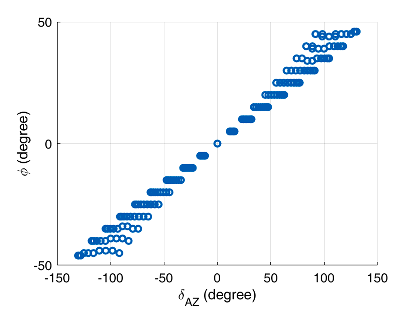
\includegraphics[width=0.4\linewidth]{Fig-naun_3a.eps}} ~~~
  \subfigure[]{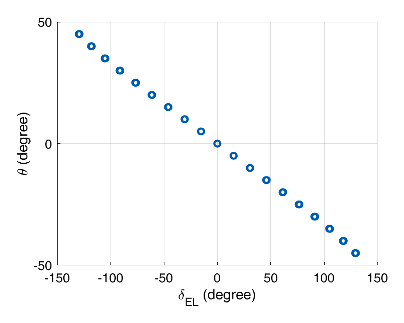
\includegraphics[width=0.4\linewidth]{Fig-naun_3b.eps}}\\
  \caption{Correlation of the (a) Azimuth angle ($\phi$) with $\delta_{AZ}$ and (b) Elevation angle ($\theta$) with $\delta_{EL}$} \label{fig_5_3}
\end{figure}

The sign of the correlation depends on the choice of the coordinate system. Here, the elevation angle is positive towards the top and negative towards the bottom and therefore a positive correlation is observed. The azimuth angle, on the other hand, is positive towards the right and negative towards the left leading to a negative correlation.

\subsection{Mapping the Radiation Angle to the Progressive Phase Shift using ANN}
From Fig. \ref{fig_5_3} (a) it is observed as $\delta_{AZ}$ and $\delta_{EL}$ is varied from -135 degree to +135 degree, the corresponding values of $\phi$ and $\theta$ vary from -45 degree to +45 degree. The elevation component of the radiation pattern shows a consistent linear correlation with the value of $\delta_{EL}$. However, the relation between $\theta$ and $\delta_{AZ}$ is not consistent. It is evident from this observation that the value of $\theta$ depends upon both $\delta_{AZ}$ and $\delta_{EL}$.

For modeling such systems, computational approaches are more suitable than analytical approaches since the computational models can detect hidden patterns in the data that cannot be observed or modeled analytically \cite{simDrivOptBook}. An artificial neural network (ANN) model is trained to map the angle of the major lobe ($\phi$, $\theta$) with the progressive phase angle ($\delta_{AZ}$, $\delta_{EL}$). The architecture of the ANN model is shown in Fig. \ref{fig_5_4}.

\begin{figure}
  \centering
  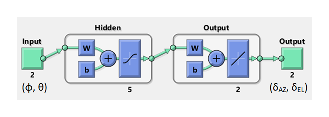
\includegraphics[width=0.6\linewidth]{Fig-naun_4.eps}\\
  \caption{Architecture of the ANN model to map the radiation angles ($\phi$, $\theta$) with the progressive phase angle ($\delta_{AZ}$, $\delta_{EL}$)} \label{fig_5_4}
\end{figure}

The ANN model is trained with the data set prepared for observing the correlation. Since the dataset is relatively small, a shallow network with 5 neurons in the hidden layer is selected for this purpose. The dataset is randomly split into test data and train data. The network is trained with a Bayesian Regularization algorithm which is suitable for smaller datasets \cite{bayesian_regularization, kumaresh_surrgoate}.

The error histogram of the neural network training is shown in Fig. \ref{fig_5_5}. A peak error of $\pm$1.15 degree is observed which is acceptable for this problem.

\begin{figure}
  \centering
  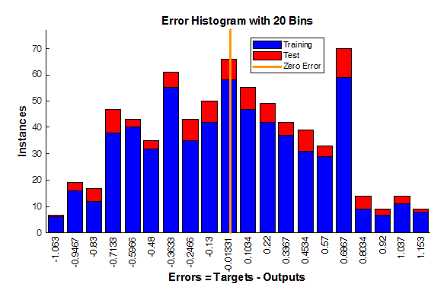
\includegraphics[width=0.5\linewidth]{Fig-naun_5.eps}\\
  \caption{Error histogram of the trained neural network} \label{fig_5_5}
\end{figure}

\subsection{Synthesis of Sparse Array}\label{c5sec_synth}
The key challenge in synthesizing a sparse scan-array is to ensure that the PSLL is minimized for all possible scan-angles or all possible combinations of $\delta_{AZ}$ and $\delta_{EL}$. Calculating the radiation pattern for all possible combinations is computationally very expensive. To make the experiment feasible, the radiation pattern is computed for three randomly selected ($\phi$, $\theta$) pairs. For each of these pairs, the corresponding values of $\delta_{AZ}$ and $\delta_{EL}$ are obtained from the trained ANN model. The radiation pattern of the antenna is computed for each of these three ($\phi$, $\theta$) pairs. The excitation weight matrix, W of the URA is calculated using Eq. \ref{c5_eq1}. The objective function returns the maximum PSLL value out of the three ($\phi$, $\theta$) pairs.

This step makes the objective function computationally expensive. To compensate for this, the PSO algorithm is used. The PSO is a widely used bio-inspired optimization algorithm and it is computationally less expensive than genetic algorithms (GA) as it requires fewer iterations \cite{pso_vs_ga}.

\begin{figure}
  \centering
  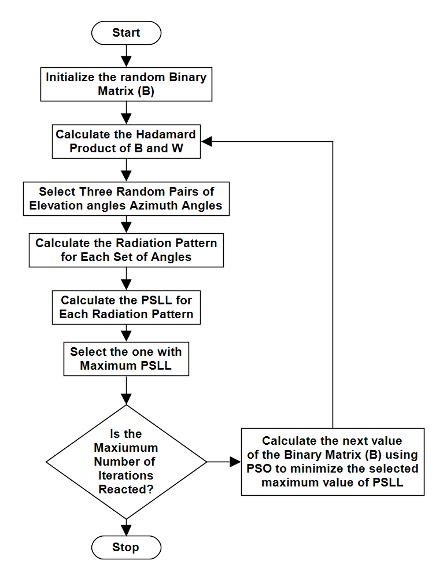
\includegraphics[width=0.5\linewidth]{Fig-naun_6.eps}\\
  \caption{Flow diagram of the sparse array synthesis steps using PSO} \label{fig_5_6}
\end{figure}

The flowchart of the proposed approach for sparse array synthesis using PSO is shown in Fig. \ref{fig_5_6}. Here, W is the excitation weight matrix of the $16\times 16$ URA. B is a binary matrix of size $16\times 16$. The weight of the sparse array is given by the Hadamard product of B and W ($B \odot W$). Thus, the optimization problem can be defined mathematically as:

\begin{equation} \label{eq_5_2}
Minimize~~F[B \odot W]
\end{equation}

Where F is the function that yields the maximum PSLL of the three randomly selected ($\phi$, $\theta$) pairs. In order to make sure that exactly 50\% of the elements are removed by the PSO, an additional constraint is added which is given by Eq. \ref{eq_5_3}.

\begin{equation}\label{eq_5_3}
\sum_{i,j}{\left[B_{i,j}\right]_{N\times N}} = \frac{N}{2}
\end{equation}

\section{Experimental Results and Discussion}\label{c5sec_res}
The $16\times 16$ URA is thinned into a sparse array using the method discussed in Section \ref{c5sec_synth}. In this section, the results of various experiments performed are covered to validate the accuracy of the proposed technique.

\subsection{The Architecture of the Sparsed Array}
The element positions of the synthesized sparse array are shown in Fig. \ref{fig_5_7}. Here, the number of elements in the sparse array is 128. The original $16\times 16$ URA has 256 elements. Thus, the number of elements in the array is reduced by 50\%.

\begin{figure}
  \centering
  
\includegraphics[width=0.4\linewidth]{Fig-naun_7.eps}\\
  \caption{Element positions of the synthesized sparse array.} \label{fig_5_7}
\end{figure}

It is observed that at some parts of the synthesized array, the vertical spacing of the original URA is maintained whereas, in some other parts, the horizontal spacing is maintained. This architecture guarantees that the excitation weights calculated for the URA work for the sparse array as well. Moreover, the elements that are scattered do not form any regular pattern. This suppresses the possibility of larger side-lobes that appear at multiples of the desired values of $\phi$ and $\theta$. It is difficult to obtain such solutions analytically.

\subsection{Analysis of the Direction of Main Lobe and PSLL}
The radiation patterns of the synthesized sparse array are analyzed for many combinations of the ($\phi$, $\theta$) pair. A part of these results is shown in Table \ref{tab_5_1}. The table shows the required values of $\phi$ and $\theta$, obtained values of $\phi$ and $\theta$, and the PSLL values of the URA and the sparse array.

\begin{table}[]
\caption{Some of the angles considered} \label{tab_5_1}
\centering
\resizebox{0.9\textwidth}{!}{%
\scriptsize
\begin{tabular}{|l|l|l|l|l|l|}
\hline
$\phi$ (deg) Desired & $\theta$  (deg) Desired & $\phi$ (deg) Obtained & $\theta$ (deg) Obtained & PSLL (dB) URA & PSLL (dB) Sparse \\ \hline
0 & 0 & 0 & 0 & -13.58 & -12.69 \\ \hline
0 & 45 & 0 & 45 & -11.64 & -11.59 \\ \hline
45 & 0 & 46 & 0 & -11.48 & -12.48 \\ \hline
45 & -45 & 45 & -45 & -10.38 & -9.89 \\ \hline
20 & 30 & 20 & 30 & -12.27 & -12.98 \\ \hline
-20 & 30 & -20 & 30 & -12.27 & -12.02 \\ \hline
-35 & -45 & -35 & -45 & -11.00 & -11.23 \\ \hline
10 & -45 & 10 & -45 & -11.60 & -11.73 \\ \hline
-10 & -40 & -10 & -40 & -11.85 & -11.75 \\ \hline
-30 & 40 & -30 & 40 & -11.58 & -11.98 \\ \hline
\end{tabular}%
}
\end{table}

It is observed that the values of $\phi$ and $\theta$ obtained are almost the same as the required values of the parameters. This observation validates the accuracy of the ANN model to predict the values of $\delta_{AZ}$ and $\delta_{EL}$. It also validates how the problem is formulated where the excitation weights of the sparse array are obtained from the Hadamard product of the weight matrix, W of the URA, and the binary matrix B.

The PSLL values are obtained from the normalized radiation pattern of the arrays. It is observed that the PSLL values of the sparse array are close to that of the original URA. Thus, there is no significant increase in the side-lobe level due to thinning the array. Fig. \ref{fig_5_8} shows the normalized radiation pattern of the antenna at $\phi$ = 30 degree and $\theta$ = 40 degree. For easier comparison, the values where the values of the radiation pattern are less than -- 60 dB are flattened.

\begin{figure}
  \centering
  \subfigure[]{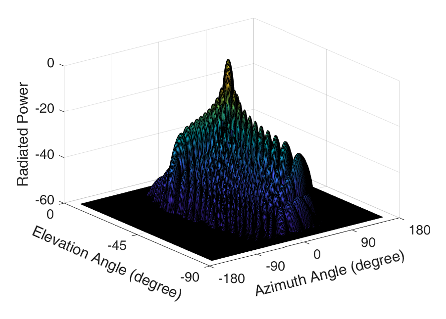
\includegraphics[width=0.4\linewidth]{Fig-naun_8a.eps}} ~~~~
  \subfigure[]{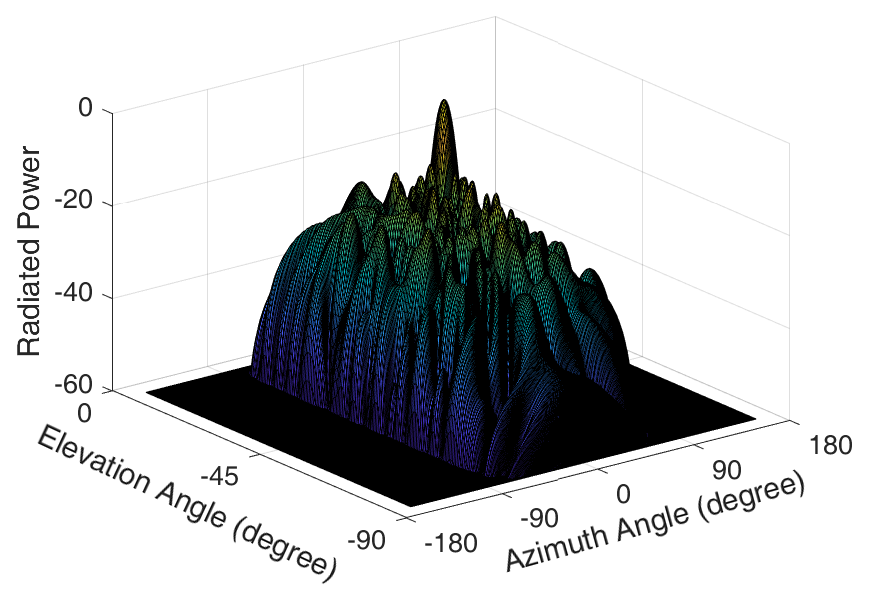
\includegraphics[width=0.4\linewidth]{Fig-naun_8b.eps}}\\
  \caption{The radiation pattern of the (a) URA and (b) the synthesized sparse array for $\phi$ = 30 degree and $\theta$ = 40 degree} \label{fig_5_8}
\end{figure}

From these figures, it is observed that the width and positions of the main lobe are identical for the URA and the sparse array. Although the sparse array has a larger number of side lobes, the values of these lobes are very small. Since the objective of the optimization problem was to suppress the PSLL only, the other side lobes are not significantly reduced.

It is not possible to include all the radiation patterns in this paper. Therefore, the overall PSLL values of the URA and the proposed sparse array are compared in a 3D surface plot shown in Fig. \ref{fig_5_9}. Here the values of $\phi$ and $\theta$ are tuned over the range of -- 45 degree to + 45 degree. It is observed that only at these two extreme points, the PSLL value of the sparse array is slightly higher than that of the original URA. As the $\phi$ and $\theta$ approach (0, 0), the values of the PSLL of the URA and sparse array become almost the same.

\begin{figure}
  \centering
  \subfigure[]{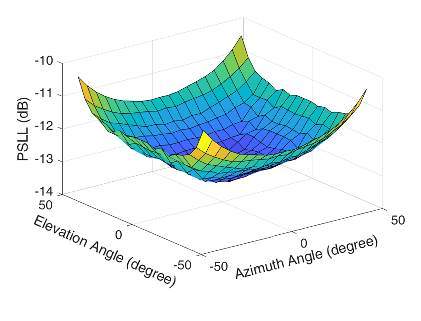
\includegraphics[width=0.4\linewidth]{Fig-naun_9a.eps}} ~~~~
  \subfigure[]{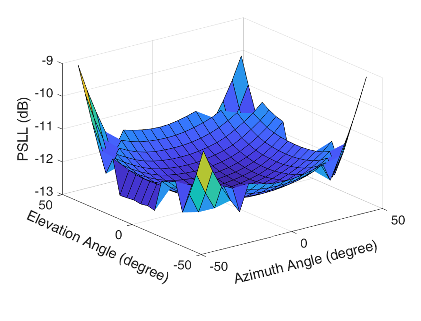
\includegraphics[width=0.4\linewidth]{Fig-naun_9b.eps}}\\
  \caption{Variation of PSLL with the direction of the main lobe for (a) URA (b) the sparse array} \label{fig_5_9}
\end{figure}

\subsection{Analysis of the Peak Gain}

This section compares the gains of the original URA and the sparse array for all the possible angles of the elevation plane and the azimuthal plane ranging from -- 45 degree to 45 degree. From Fig. \ref{fig_5_10}, it is observed that as the distribution of the gains with the angle of the main lobe shows a similar trend for both the original URA and the sparse array. The difference in gain is maximum at the edges and reduces as the azimuth and elevation angles are close to zero. The difference in gain observed is 2 dB whereas the maximum difference is 4.5 dB.

\begin{figure}
  \centering
  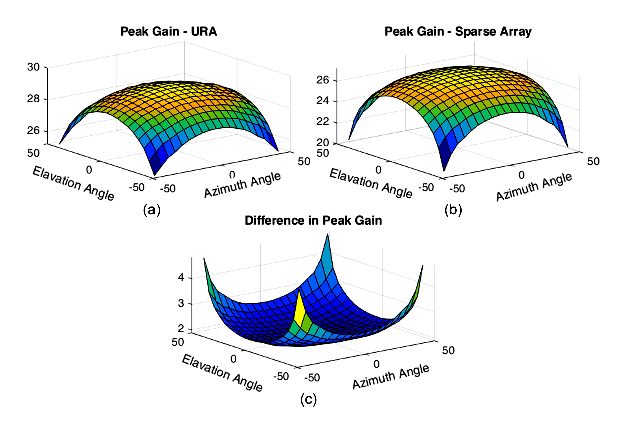
\includegraphics[width=0.95\linewidth]{Fig-naun_10.eps}\\
  \caption{(a) Distribution of the peak gain of the URA, (b) Distribution of the peak gain of the sparse array, (c) Difference between peak gains of URA and Sparse array} \label{fig_5_10}
\end{figure}

It is evident from the experimental results that the gain of the antenna gets reduced as the number of elements of the array is decreased. This is an intrinsic limitation of sparse array \cite{sparse_rect_planar}. There have been approaches for addressing this issue which include altering the physical structure of the elements of the array to compensate for the reduction in gain \cite{compact_sparse_array_satcom}. The present work has a future scope of improvement in this direction.

\subsection{Analysis of the Beam-width}
The beam-width is another important factor to be considered when a sparse array is synthesized. The beam-width and PSLL are often considered related constraints in many applications \cite{arrayTradeoffs}. The beam-widths of the original URA and the synthesized sparse scan-array are plotted for azimuth angles and elevation angles in the range from -- 45 degree to 45 degree in Fig. \ref{fig_5_11}.

\begin{figure}
  \centering
  \includegraphics[width=0.95\linewidth]{Fig-naun_11.eps}\\
  \caption{Distribution of the beam-width for (a) the original URA and (b) the synthesized sparse array} \label{fig_5_11}
\end{figure}

\begin{figure}
  \centering
  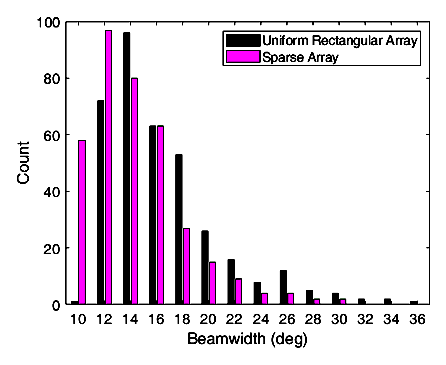
\includegraphics[width=0.5\linewidth]{Fig-naun_12.eps}\\
  \caption{Histogram of the beam widths of the URA and the sparse planar array.} \label{fig_5_12}
\end{figure}

From Fig. \ref{fig_5_11} (a) and (b) it is observed that the beam-width of the two arrays exhibit almost similar variations with the scan-angles. The maximum beam-width of the URA is 36 degree whereas that of the sparse array is 29 degree. The histogram of the beam-widths of the two arrays is shown in Fig. \ref{fig_5_12}. The sparse array has more scan-angles where the beam width is between 10-12 degrees. Beyond the beam-width of 16 degree, the number of points is lower in case of the sparse array as compared to the URA. It infers that the sparse array has narrower beam-widths than the URA.

\section{Conclusion} \label{c5sec_cncl}
A technique for synthesizing a sparse array from a $16\times 16$ URA is presented. The excitation weight matrix, W of the URA are estimated using an ANN model from the desired scan-angle. The PSO is used for obtaining a binary matrix B, such that the Hadamard product of B and W yields the excitation weights of the sparse antenna array. The experimental results show that the desired scan-angles of the sparse array are accurately obtained using this technique.

The PSLL of the URA and the sparse array are compared for all possible scan-angles in a range of -- 45 degree to + 45 degree for both the elevation plane and the azimuthal plane. It is observed that the PSLL of the synthesized sparse array is almost the same as that of the URA except at the extreme ends of the scanning range.

The overall scan angle of the proposed antenna array is 90 degree for both the azimuth plane and the elevation plane. The array comprises cosine antenna elements that represent printed antennas used in 5G millimeter-wave wireless communication. A comparative analysis of the original URA and the sparse array is observed in terms of gain and beam-width. It is observed that although there is a slight reduction in the gain of the sparse array, the beam-width is less indicating a better resolution for radar or directional wireless communication.

There have been a reduction in gain of the array as the number of elements is reduced. This is a common problem experienced with sparse arrays. There have been approaches proposed for addressing this issue. However, it is difficult to frame such an objective in the current construct of the optimization problem.
